

% Kun käytät tätä, älä lataa pakettia stfloats tai fix2col. Tämä lataa
% myös paketin fixltx2e.
%% "When the new output routine for LaTeX3 is done, this package will
%% be obsolete. The sooner the better..."
\RequirePackage{dblfloatfix}
% Kun käytät tätä, et enää tarvitse paketteja type1cm ja type1ec:
\RequirePackage{fix-cm}

% Helpottaa pdf(la)tex:in läsnäolon tarkistusta if-lauseilla
\RequirePackage{ifpdf}

\documentclass[a4paper,onecolumn,12pt,finnish,oneside,final]{boek3}

\setcounter{secnumdepth}{7}

%%%%%%%%%%%%%%%%%%%%%%%%%%%%%%%%%%%%%%%%%%%%%%%%%%%%%%%%%%%%%%%%%%%%%%%%%
% Suometus ja fontit
\usepackage[utf8]{inputenc}

% cmap: "Make the PDF files generated by pdflatex "searchable and copyable"
% in Adobe (Acrobat) Reader and other compliant PDF viewers."
% (Pakko olla ennen fontenc-pakettia)
\ifpdf % Eräillä saattaa olla buginen cmap. Yritetään välttää sitä.
\usepackage{cmap}
\fi

\usepackage[T1]{fontenc}
% Suometusten asettaminen jatkuu myöhemmin

\usepackage{blindtext}
\usepackage{lipsum}

%%%%%%%%%%%%%%%%%%%%%%%%%%%%%%%%%%%%%%%%%%%%%%%%%%%%%%%%%%%%%%%%
% Fontit
%

% Yleisimmät erikoismerkit, kuten copyleft
\usepackage{textcomp}

%%% Matikkafontteja

% Matikka-symboleita
\usepackage{latexsym}

% AMS:sän matikka-paketteja:
% Lisätietoa paketista optiolla "?"
%\usepackage[?]{amsmath}
\RequirePackage{amsmath}
\RequirePackage{amsfonts}
\RequirePackage[psamsfonts]{amssymb}
\RequirePackage{amsxtra}
\RequirePackage{amscd}
\RequirePackage{amsthm}
\RequirePackage{mathrsfs}

% Math fonts 
\usepackage{arevmath}

% Text fonts
\usepackage{dejavu}

\renewcommand{\familydefault}{\sfdefault}
\fontfamily{\familydefault}

\usepackage{titlesec}

%\titleformat{\part}[display]
%  {\normalfont\Huge\filright\bfseries}{\MakeUppercase{Osa\ \thepart}}{\Huge\filright\MakeUppercase}

\titleformat{\part}
  {\normalfont\filright\Huge\bfseries\rmfamily}{Osa \thepart}{1em}{}

%\titleformat{\chapter}[display]
%  {\normalfont\huge\filright\bfseries}{\MakeUppercase{\chaptertitlename\ \thechapter}}{\Huge\filright\MakeUppercase}

\titleformat{\chapter}
  {\normalfont\filright\huge\bfseries\rmfamily}{\chaptertitlename\ \thechapter}{1em}{}

\titleformat{\section}
  {\normalfont\filright\LARGE\bfseries\rmfamily}{\thesection}{1em}{}

\titleformat{\subsection}
  {\normalfont\filright\Large\bfseries\rmfamily}{\thesubsection}{1em}{}

\titleformat{\subsubsection}
  {\normalfont\filright\large\bfseries\rmfamily}{\thesubsubsection}{1em}{}

\titleformat{\paragraph}[runin]
  {\normalfont\normalsize\bfseries\rmfamily}{\theparagraph}{1em}{}

\titleformat{\subparagraph}[runin]
  {\normalfont\normalsize\bfseries\rmfamily}{\thesubparagraph}{1em}{}




% Tukea pdf(la)texin microtypes-laajennoksille. Pakko olla
% fonttimäärityksien jälkeen.
\ifpdf
\usepackage[protrusion=true,expansion=true,verbose=true]{microtype}
\else
\usepackage[verbose=true]{microtype}
\fi


\makeatletter
\g@addto@macro\verbatim{\pdfprotrudechars=0 \pdfadjustspacing=0\relax}
\makeatother




% Fontit asetettu!

% Loput suometukset (mutta myös enkunkieltä saatetaan tarvita):
\usepackage[finnish,english]{babel}
%\usepackage[finnish]{babel}

% Suometukset asetettu!

% if-then-else-rakenteita helposti
\usepackage{ifthen}

% Lisää kokomäärityksiä:
\usepackage[12pt]{moresize}

% Tee jotain jokaisen sivun kohdalla:
% (totpages tarvii tätä)
\usepackage{everyshi}

% Värien tuki:
% (Mihinkähän mä tätä tarvitsinkaan?)
%\usepackage{color}

% Kuvien lisäys dokumenttiin:
% (Mihinkähän mä tätä tarvitsinkaan?)
%\usepackage{graphicx}

% Laskutehtävien suoritusta (geometry-paketti hyötyy tästä):
\usepackage{calc}


\usepackage[nomarginpar,includeheadfoot]{geometry}

% vasen marginaali
\geometry{lmargin=4.0cm}
% oikea marginaali
\geometry{rmargin=2.0cm}
% ylämarginaali
\geometry{tmargin=2.0cm}
% alamarginaali
\geometry{bmargin=2.0cm}


%%%%%%%%%%%%%%%%%%%%%%%%%%%%%%%%%%%%%%%%%%%%%%%%%%%%%%%%%%%%%%%%
% Ykkösvälike, puolitoistakertainen välike ja kakkosvälike yms.
\usepackage{setspace}
%\singlespacing
\onehalfspacing
%\spacing{1.7} % Tämä bugasi joskus aiheuttaen tällaista: (\end occurred inside a group at level 1) 
%\doublespacing

% URL:ien ladonta ja "tavutus"
\usepackage[obeyspaces,spaces,hyphens,T1]{url}
%\renewcommand\url{\begingroup \def\UrlLeft{<URL: }\def\UrlRight{>}\urlstyle{rm}\Url}
%\def\UrlBigBreakPenalty{120}
%\def\UrlBreakPenalty{200}

% Helpottaa TeX:iin liittyvien nimien ladontaa (LaTeX, BibTeX jne.)
\usepackage{texnames}

%%%%%%%%%%%%%%%%%%%%%%%%%%%%%
% Upeet headerit ja footerit





% Ei sisennetä kappaleen ekaa riviä
\setlength{\parindent}{0.0cm}


\ifpdf % We are running pdftex
\pdfcompresslevel=9
\pdfpkresolution=1200
\fi

\usepackage{tikz}
\usetikzlibrary{calc}

\begin{document}

\selectlanguage{finnish}

\begin{titlepage}

  \begin{center}
    \begin{doublespace}
      \begin{LARGE}
        \textrm{Tekijätiimin nimi} \\
      \end{LARGE}
      
      \vspace{0.5cm}
      \hrule height 2pt
      \vspace{1cm}
      \begin{Huge}
        \textbf{\textrm{Otsikko}}
      \end{Huge}
      
      \vfill
      
      \begin{huge}
        \textrm{Alaotsikko}
      \end{huge}
      \vspace{1cm}
      \hrule height 2pt
    \end{doublespace}
  \end{center}
  
  \vfill
  \begin{flushright}
    \textbf{Sekalaista \\
      muuta asiaa \\
      sisällöstä \\
    }
  \end{flushright}
  
\end{titlepage}

\tableofcontents




\part{Puhtauspalvelualan matematiikkaa}

\chapter{Foo}

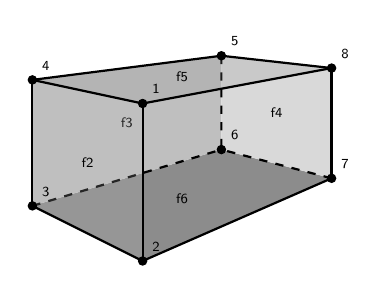
\begin{tikzpicture}
	%%% Edit the following coordinate to change the shape of your
	%%% cuboid
      
	%% Vanishing points for perspective handling
	\coordinate (P1) at (-7cm,1.5cm); % left vanishing point (To pick)
	\coordinate (P2) at (8cm,1.5cm); % right vanishing point (To pick)

	%% (A1) and (A2) defines the 2 central points of the cuboid
	\coordinate (A1) at (0em,0cm); % central top point (To pick)
	\coordinate (A2) at (0em,-2cm); % central bottom point (To pick)

	%% (A3) to (A8) are computed given a unique parameter (or 2) .8
	% You can vary .8 from 0 to 1 to change perspective on left side
	\coordinate (A3) at ($(P1)!.8!(A2)$); % To pick for perspective 
	\coordinate (A4) at ($(P1)!.8!(A1)$);

	% You can vary .8 from 0 to 1 to change perspective on right side
	\coordinate (A7) at ($(P2)!.7!(A2)$);
	\coordinate (A8) at ($(P2)!.7!(A1)$);

	%% Automatically compute the last 2 points with intersections
	\coordinate (A5) at
	  (intersection cs: first line={(A8) -- (P1)},
			    second line={(A4) -- (P2)});
	\coordinate (A6) at
	  (intersection cs: first line={(A7) -- (P1)}, 
			    second line={(A3) -- (P2)});

	%%% Depending of what you want to display, you can comment/edit
	%%% the following lines

	%% Possibly draw back faces

	\fill[gray!90] (A2) -- (A3) -- (A6) -- (A7) -- cycle; % face 6
	\node at (barycentric cs:A2=1,A3=1,A6=1,A7=1) {\tiny f6};
	
	\fill[gray!50] (A3) -- (A4) -- (A5) -- (A6) -- cycle; % face 3
	\node at (barycentric cs:A3=1,A4=1,A5=1,A6=1) {\tiny f3};
	
	\fill[gray!30] (A5) -- (A6) -- (A7) -- (A8) -- cycle; % face 4
	\node at (barycentric cs:A5=1,A6=1,A7=1,A8=1) {\tiny f4};
	
	\draw[thick,dashed] (A5) -- (A6);
	\draw[thick,dashed] (A3) -- (A6);
	\draw[thick,dashed] (A7) -- (A6);

	%% Possibly draw front faces

	% \fill[orange] (A1) -- (A8) -- (A7) -- (A2) -- cycle; % face 1
	% \node at (barycentric cs:A1=1,A8=1,A7=1,A2=1) {\tiny f1};
	\fill[gray!50,opacity=0.2] (A1) -- (A2) -- (A3) -- (A4) -- cycle; % f2
	\node at (barycentric cs:A1=1,A2=1,A3=1,A4=1) {\tiny f2};
	\fill[gray!90,opacity=0.2] (A1) -- (A4) -- (A5) -- (A8) -- cycle; % f5
	\node at (barycentric cs:A1=1,A4=1,A5=1,A8=1) {\tiny f5};

	%% Possibly draw front lines
	\draw[thick] (A1) -- (A2);
	\draw[thick] (A3) -- (A4);
	\draw[thick] (A7) -- (A8);
	\draw[thick] (A1) -- (A4);
	\draw[thick] (A1) -- (A8);
	\draw[thick] (A2) -- (A3);
	\draw[thick] (A2) -- (A7);
	\draw[thick] (A4) -- (A5);
	\draw[thick] (A8) -- (A5);
	
	% Possibly draw points
	% (it can help you understand the cuboid structure)
	\foreach \i in {1,2,...,8}
	{
	  \draw[fill=black] (A\i) circle (0.15em)
	    node[above right] {\tiny \i};
	}
	% \draw[fill=black] (P1) circle (0.1em) node[below] {\tiny p1};
	% \draw[fill=black] (P2) circle (0.1em) node[below] {\tiny p2};
\end{tikzpicture}

\begin{align*}
2,05\ l = x\ dm^3  &\Leftrightarrow 1\ l = 1\ dm^3 \\
&\implies x = 2,05 \\
&\implies  2,05\ l = 2,05\ dm^3
\end{align*}


\begin{align*}
1\ l &= 1000\ ml \\
\frac{5400}{1000} &= 5,4 \\
\implies 5400\ ml &= 5,4\ l
\end{align*}



\begin{align*}
1\ cm^2 &= 100\ mm^2 \\
100 \cdot 300 &= 30000 \\
\implies 300\ cm^2 &= 30000\ mm^2
\end{align*}


\begin{align*}
100\ cm &= 1\ m \\
\frac{7}{100} &= 0,07 \\
\implies 7\ cm &= 0,07\ m \\
\implies 2\ m + 7\ cm &= 2\ m + 0,07\ m = 2,07\ m
\end{align*}


\begin{align*}
1\ min &= 60\ s \\
\frac{1500}{60} &= 25 \\
\implies 1500\ s &= 25\ min
\end{align*}


\begin{align*}
1\ h &= 60\ min \\
1,35 \cdot 60 &= 81 \\
\implies 1,35\ h &= 81\ min
\end{align*}


\begin{align*}
1\ l &= 10\ dl = 100\ cl \\
\frac{8}{10} &= 0,8 \\
\frac{8}{100} &= 0,08 \\
\implies 8\ dl + 8\ cl &= 0,8\ l + 0,08\ l = 0,88\ l
\end{align*}


\begin{align*}
1\ ha &= 10000\ m^2 \\
5 \cdot 10000 &= 50000 \\
\implies 5\ ha &= 50000\ m^2
\end{align*}


\chapter{Bar}

\begin{align*}
\frac{5}{475} &= 0,010526 \\
              &=  01,0526\ \%
\end{align*}



\[
180 + \left ( \frac{180}{100} \cdot 15 \right ) = 207
\]




\[
\frac{15\ kg}{20} \cdot 100 = 75\ kg
\]




\[
\frac{75}{250} = 0,3 = 30\ \%
\]


\chapter{Baz}



\begin{align*}
\frac{1500\ \text{€}}{100 + 3,5} \cdot 3,5 &= 50,724635\ \text{€}  \\
                                 &\approx 50,72\ \text{€}
\end{align*}




\begin{align*}
1500\ \text{€} - \left ( \frac{1500\ \text{€}}{100 + 3,5}  \cdot 3,5 \right ) &= 1500\ \text{€} - 50,724635\ \text{€} \\
&= 1449,275365\ \text{€}\\
&\approx 1449,28\ \text{€}
\end{align*}






\begin{align*}
1\ l &= 1000\ ml \\
\frac{5\ \text{€}}{1000} \cdot 750 &= 3,75\ \text{€}
\end{align*}




\begin{align*}
1\ l &= 10\ dl \\
\frac{41,50\ \text{€}}{5\ l} &= 8,30\ \text{€}/l \\
\frac{2,3}{10} = 0,23 \implies 2,3\ dl &= 0,23\ l \\
7\ d \cdot 0,23\ l \cdot 8,30\ \text{€}/l &= 7\ d \cdot 1,9090\ \text{€} \\
&= 13,3630\ \text{€}/viikko \\
&\approx 13,36\ \text{€}/viikko
\end{align*}


\chapter{Qux}


\begin{align*}
25\ min + 3600\ s + 3,5\ h &= \\
25 \cdot 60\ s + 3600\ s + 3,5 \cdot 60 \cdot 60\ s &= \\
1500\ s + 3600\ s + 12600\ s &= 17700\ s \\
1\ h &= 3600\ s \\
\frac{17700}{3600} &= 4,916666 \\
\implies 17700\ s &= 4,916666\ h
\end{align*}




\begin{align*}
45\ min + 7,2\ h + 5,6\ h - 2,1\ h &= \\
\frac{45}{60}\ h + 7,2\ h + 5,6\ h - 2,1\ h &= 11,45\ h
\end{align*}




\begin{align*}
23\ h + 7,8\ h + 0,7\ h = 31,5\ h
\end{align*}




\begin{align*}
3,3\ h + 45\ min - 2,6\ h &= \\
3,3\ h + \frac{45}{60}\ h - 2,6\ h &= 1,45\ h
\end{align*}


\chapter{Quux}



\begin{align*}
5\ d \cdot 40 \cdot 20\ ml &= 4000\ ml/viikko \\
                           &= 4\ l/viikko
\end{align*}




\begin{align*}
5\ d \cdot 40 \cdot 5\ ml &= 1000\ ml/viikko \\
                          &= 1\ l/viikko \\
\left ( \frac{365\ d}{7\ d} \right ) \cdot 1\ l &= 52.142857\ l/a \\
\end{align*}




\begin{align*}
52.142857\ l \cdot 3,20\ \text{€}/l &= 166,857142\ \text{€} \\
                                    &\approx 166,86\ \text{€}
\end{align*}


\chapter{Quuux}



\begin{align*}
250\ m^2 \cdot 0,18\ min/m^2 \cdot 260\ d &= 11700\ min \\
                                          &= 195\ h
\end{align*}




\begin{align*}
250\ m^2 \cdot \frac{260\ d}{2} \cdot 0,009\ min/m^2 &= 292,5\ min \\
                                                     &= 4,875\ h
\end{align*}


\part{Erilaisia sokkotekstejä}

%%% Erilaisia sokkotekstejä (Lorem ipsumia)

%%% blindtext-paketista

%\blinddocument
\Blinddocument

\chapter{Sokkotekstiä}

\section{Sokkotekstiä oletusfontilla}

\Blindtext

\section{Sokkotekstiä kirjoituskoneella}

\texttt{\blindtext}


\section{Sokkotekstiä sans-seriffillä}

\textsf{\blindtext}

\section{Sokkotekstiä seriffillä}

\textrm{\blindtext}



%%% Ei toimi tässä
%\blindmathpaper

\chapter{Lipsum}

%%% lipsum-paketista

\section{Lorem ipsum}

\lipsum[1-5]

\texttt{\lipsum[6-10]}

\textsf{\lipsum[11-15]}

\textrm{\lipsum[16-20]}

%%% Local Variables: 
%%% mode: latex
%%% End: 




\part{Edistyneempää matematiikkaa}

\chapter{Kamaa Stephen Hartkelta}

%%%%%%%%%%%%%%%%%%%%%%%%%%%%%%%%%%%%%%%%%%%%%%%%%%%%%%%%%%%%%%%%%%%%%%%%%%%%%%%%
%%%%  /usr/share/doc/texlive-fonts-extra-doc/fonts/arev/mathtesty.tex

% mathtesty.tex, by Stephen Hartke 20050522
% based on mathtestx.tex in the mathptmx package
% and symbols.tex by David Carlisle

\section{Radikaaleja}

\begin{displaymath}
  \sqrt{x+y} \qquad \sqrt{x^{2}+y^{2}} \qquad 
  \sqrt{x_{i}^{2}+y_{j}^{2}} \qquad
  \sqrt{\left(\frac{\cos x}{2}\right)} \qquad 
  \sqrt{\left(\frac{\sin x}{2}\right)}
\end{displaymath}

\begingroup
\delimitershortfall-1pt
\begin{displaymath}
  \sqrt{\sqrt{\sqrt{\sqrt{\sqrt{\sqrt{\sqrt{x+y}}}}}}}
\end{displaymath}
\endgroup % \delimitershortfall


\section{Over- and underbraces}

\begin{displaymath}
  \overbrace{x} \quad
  \overbrace{x+y} \quad
  \overbrace{x^{2}+y^{2}} \quad
  \overbrace{x_{i}^{2}+y_{j}^{2}} \quad
  \underbrace{x} \quad
  \underbrace{x+y} \quad
  \underbrace{x_{i}+y_{j}} \quad
  \underbrace{x_{i}^{2}+y_{j}^{2}} \quad
\end{displaymath}




\chapter{Teoreemoja}

%%%%%%%%%%%%%%%%%%%%%%%%%%%%%%%%%%%%%%%%%%%%%%%%%%%%%%%%%%%%%%%%%%%%%%%%%%%%%%%%
%%%% /usr/share/doc/texlive-doc/fonts/arev/fontsample.tex
%%%% /usr/share/doc/texlive-fonts-extra-doc/fonts/arev/fontsample.tex

%\theoremstyle{definition}
\newtheorem{theorem}{Theorem}


\begin{theorem}[Residue Theorem]
Let $f$ be analytic in the region $G$ except for the isolated singularities $a_1,a_2,\ldots,a_m$. If $\gamma$ is a closed rectifiable curve in $G$ which does not pass through any of the points $a_k$ and if $\gamma\approx 0$ in $G$ then
\[
\frac{1}{2\pi i}\int_\gamma f = \sum_{k=1}^m n(\gamma;a_k) \text{Res}(f;a_k).
\]
\end{theorem}

Another nice theorem from complex analysis is

\begin{theorem}[Maximum Modulus]
Let $G$ be a bounded open set in $\mathbb{C}$ and suppose that $f$ is a continuous function on $G^-$ which is analytic in $G$. Then
\[
\max\{|f(z)|:z\in G^-\}=\max \{|f(z)|:z\in \partial G \}.
\]
\end{theorem}

\newcommand{\abc}{abcdefgh\hbar\hslash i\imath j\jmath klmnopqrstuvwxyz}
\newcommand{\ABC}{ABCDEFGHIJKLMNOPQRSTUVWXYZ}
\newcommand{\alphabeta}{\alpha\beta\varbeta\gamma\delta\epsilon\varepsilon\zeta\eta\theta\vartheta\iota\kappa\varkappa\lambda\mu\nu\xi o\pi\varpi\rho\varrho\sigma\varsigma\tau\upsilon\phi\varphi\chi\psi\omega}
\newcommand{\AlphaBeta}{\Gamma\Delta\Theta\Lambda\Xi\Pi\Sigma\Upsilon\Phi\Psi\Omega}



%%%%%%%%%%%%%%%%%%%%%%%%%%%%%%%%%%%%%%%%%%%%%%%%%%%%%%%%%%%%%%%%%%%%%%%%%%%%%%%%
%%%% /usr/share/doc/texlive-doc-en/fonts/free-math-font-survey/source/textfragment.tex

\chapter{Lisää kamaa}

\ABC \quad $\ABC$

$\mathrm{A} \Lambda \Delta \nabla \mathrm{B C D} \Sigma \mathrm{E F} \Gamma \mathrm{G H I J K L M N O} \Theta \Omega \mho \mathrm{P} \Phi \Pi \Xi \mathrm{Q R S T U V W X Y} \Upsilon \Psi \mathrm{Z} $  $ \quad 1234567890 $

% don't allow overfull boxes
{\par \tolerance=0 \emergencystretch=100em
 $a\alpha b \beta c \partial d \delta e \epsilon \varepsilon f \zeta \xi g \gamma h \hbar \hslash \iota i \imath j \jmath k \kappa  \linebreak[3]
 \varkappa l \ell \lambda m n \eta \theta \vartheta o \sigma \varsigma \phi \varphi \wp p \rho \varrho q r s t \tau \pi u \mu \nu v \linebreak[3]
  \upsilon w \omega \varpi x \chi y \psi z$ $\infty \propto \emptyset
  \varnothing \mathrm{d}\eth \backepsilon  \linebreak[3] $\par}




%%%%%%%%%%%%%%%%%%%%%%%%%%%%%%%%%%%%%%%%%%%%%%%%%%%%%%%%%%%%%%%%%%%%%%%%%%%%%%%%
%%%% http://milde.users.sourceforge.net/Matheschriften/lxfonts-test.tex
%%%% http://milde.users.sourceforge.net/Matheschriften/mathfonttest.tex

\chapter{Vielä lisää kamaa}


\begin{equation}
\sqrt{a+b}\ne\sqrt{a}+\sqrt{b}\quad
\mbox{und}
\quad\sqrt{\frac{a}{b}}\ne\frac{\sqrt{a}}{\sqrt{b}}.
\end{equation}



\end{document}



%%% Local Variables: 
%%% mode: latex
%%% End: 


\end{document}

% -*- coding: utf-8 -*-

%%% Local Variables: 
%%% mode: latex
%%% TeX-master: t
%%% coding: utf-8
%%% End: 

